% !TeX root = ../DistributedConsensus.tex
% !TeX spellcheck = en_GB
\chapter{Validation and Consensus of Histories}
\label{chap:consensusindcr}
	This chapter defines how histories from malicious events are identified and removed as well as how correctly functioning events can agree upon an order of execution.
	
	\newpar In distributed systems malicious agents are introduced. These agents can take many forms and corrupt data in many ways. Therefore it is wanted to have a mechanism which can observe, identify, and handle these corruptions in a predictable way. Traditionally malicious agents can tamper with messages in transfer by; altering messages, replaying messages and withholding messages. We assume that any of these kinds of corrupting messages in transfer is not present in this system. How a system can handle these kinds of corruption is examined in \todo[inline]{Henvis til en artikel der udforsker disse traditionelle typer "snyd"}.
	
	\newpar Therefore the kinds of cheating which is examined in this project is the following:
	\begin{definition}
		\textbf{Cheating} is any changing of a history that is not corresponding to what actually happened in the DCR graph.
	\end{definition}
	\todo[inline]{Tilføj rigtig definition.}
	
	\section{Validating histories}
	In order to identify malicious events in a given history, we need to define what a valid history is:
	
		\begin{definition}
			A \textit{\textbf{Valid History}} is a history, H, for which it applies that all actions happen according to the rules of the DCR graph, abiding serial equivalence and being in a strict partial order. 
		\end{definition}
		
	This also introduces a special kind of cheating:
	
		\begin{definition}
			\textbf{Inconsistent cheating} is the act of manipulation  in a way where the history is not valid.
		\end{definition}
		
	\subsection{DCR Rules}
	A given execution must abide the rules of the DCR graph it is part of. That includes the following:
	
	\newpar \textbf{Valid relations}: A given history for an event, $e1$, must only contain actions which represents relations to another event, $e2$, where there exists such a relation in the DCR graph definition and vice versa. 
	
	\newpar \textbf{Complete executions}: A given event, $e1$ must affect all of its outgoing relations when executing. Furthermore every event that $e1$ has a relation to must have a \texttt{By} relation in its history after $e1$ has executed.
	
	\newpar \textbf{Executions only in Valid States}: A given history for an event, $e1$, must only have executions where the state is included, and the event's conditions are either executed or excluded.
	
	\subsection{Serial Equivelence Rules}
	A given execution must abide the rules of serially equivelence. That includes the following:
	
	\newpar \textbf{Non-disrupted Executions}: A given event, $e1$ must affect all of its outgoing relations when executing without having any other executions start or affect the event. The exception to the rule is when an event has a relation to itself in which case a \texttt{By} action is allowed.
	
	\newpar \textbf{Wait for Complete Execution}: A given event, $e1$ must be affected by all the its ingoing relations from event, $e2$ when $e2$ executes, before anything else happens. The exception to the rule is when an event has a relation to itself in which case a actions from the execution are allowed before the next \texttt{By} action happens. 
	
	\subsection{History Graph Rules / Strict Partial Ordering / Lamport Logical Clocks}
	A given history must abide the rules of being a strict partial order. That includes the following:
	
	\newpar \textbf{Total Order of Local Timestamps}: A history of an event $e1$ must have its local timestamps be in strict total order.
	
	\newpar \textbf{Total Order of Counterpart Timestamps}: In the history of $e1$ actions with counterpart id $e2$ must have its counterpart timestamp in strict total order.  The exception to the rule is when an event has a relation to itself in which case counterpart timestamp can be be lower. \todo{example}
	
	\newpar \textbf{Outgoing Relations Timestamp Order}: When an action is part of an outgoing relation the counterpart's \texttt{By} action's timestamp must be higher than the outgoing one. 
	
	\newpar \textbf{Mismatches in typestamps:} A given history graph must not contain any actions that have relations to actions with an invalid timestamp. This would imply that either an executing event has tampered with its outgoing action history or that an event affected by an execution has tampered with its ingoing action history. 
	
	\newpar These rules together makes sure that no cycles can exist.
	
	\todo[inline]{Maybe remove next paragraph}
	\textbf{Cycles:} A given history graph must not contain any cycles, since cycles in the history graph would imply that an action, $a1$, has occurred before another action, $a2$, but $a2$ has also occurred before $a1$. This is not possible in any execution, and a given history with cycles will therefore be invalid.
	
	
	
	\todo[inline]{Uddyb regler og tilføj evt. en figur der viser mismatches mellem timestamps. }
	
	\todo[inline]{Uddyb regler og tilføj evt. en figur der viser invalid DCR historik ift. relations der ikke eksisterer. }
	
	\subsection{Simulation}
	Executions only in Valid States is a special case which is non trivial to check. HOW DO WE DO. ALSO WE DONT KNOW IF IT IS THE EVENT ITSELF DOING BAD BEHAVIOR OR A CONDITION REPLIED WITH LYING DATA.
	
	\newpar If any of these rules are not adhered to an event must be malicious, since any well functioning event would not be able to such a create history. Thereby allowing us to identify and if wanted remove this subset of Corruption types 
	
	\section{Consistent cheating}
	Until now we have examined inconsistent cheating, but malicious events are also able to cheat consistently:
	\begin{definition}
		\textbf{Consistent cheating} is the act of manipulating data in a way where the history is still valid.
	\end{definition}
	
	\newpar Consistent cheating can take a number of forms:
	

	\newpar \textbf{Non correct timestamps}: A malicious event manipulates the timestamps of the actions in the history, while still mainting order in both local and counterpart timestamps.
	
	\newpar \textbf{Non correct number of executions}: A malicious event which is executable executes either fewer or more times than it has done.
	\todo[inline]{more types?}
	
	\subsection{Cases}
	Detecting and identifying consistently cheating events is difficult, due to the fact that it is not possible to look at a single event's history and determine if it is valid or not. We will now examine how the structure of the DCR graph, and the connecting between malicious events contribute to the ability to detect and identifying the cheating.
	
	\newpar \textbf{Single Malicious Event}: 
	
	\begin{figure}[H]
		\centering
		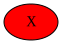
\includegraphics[]{6consensus/images/1.pdf}
		\caption{}
		\label{fig:consensus:single}
	\end{figure}
	
	\newpar \textbf{Single Malicious Event With Relation to Self}:
	
	\begin{figure}[H]
		\centering
		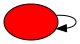
\includegraphics[]{6consensus/images/5.pdf}
		\caption{}
		\label{fig:consensus:single}
	\end{figure}
	
	\newpar \textbf{Single Malicious Event With Relation to Good Event}:
	 
	\begin{figure}[H]
		\centering
		\includegraphics[]{6consensus/images/3.pdf}
		\caption{}
		\label{fig:consensus:single}
	\end{figure}
	
	\newpar \textbf{Good Event With Relation to Single Malicious Event}:
	 
	\begin{figure}[H]
		\centering
		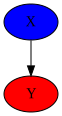
\includegraphics[]{6consensus/images/2.pdf}
		\caption{}
		\label{fig:consensus:single}
	\end{figure}
	
	\newpar \textbf{Good and Malicious Event with Relations to eachother}:
	
	\begin{figure}[H]
		\centering
		\includegraphics[]{6consensus/images/6.pdf}
		\caption{}
		\label{fig:consensus:single}
	\end{figure}
	
	\newpar \textbf{Malicious Event A with relation to Malicious Event B}: 
	
	\begin{figure}[H]
		\centering
		\includegraphics[]{6consensus/images/4.pdf}
		\caption{}
		\label{fig:consensus:single}
	\end{figure}
	
	\newpar \textbf{Two Malicious Events With Relations To Eachother}:
	
	\begin{figure}[H]
		\centering
		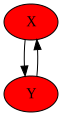
\includegraphics[]{6consensus/images/7.pdf}
		\caption{}
		\label{fig:consensus:single}
	\end{figure}
